% !TeX root=../journalDeepMedic.tex

\section{Introduction}

Segmentation and the subsequent quantitative assessment of lesions in medical images provide valuable information for the analysis of neuropathologies and are important for planning of treatment strategies, monitoring of disease progression and prediction of patient outcome. For a better understanding of the pathophysiology of diseases, quantitative imaging can reveal clues about the disease characteristics and effects on particular anatomical structures. For example, the associations of different lesion types, their spatial distribution and extent with acute and chronic sequelae after traumatic brain injury (TBI) are still poorly understood (\cite{Maas2015}). However, there is growing evidence that quantification of lesion burden may add insight into the functional outcome of patients (\cite{Ding2008,Moen2012}). Additionally, exact locations of injuries relate to particular deficits depending on the brain structure that is affected (\cite{lehtonen2005neuropsychological, Warner2010d, Sharp2011}). This is in line with estimates that functional deficits caused by stroke are associated with the extent of damage to particular parts of the brain (\cite{carey2013beyond}). Lesion burden is commonly quantified by means of volume and number of lesions, biomarkers that have been shown to be related to cognitive deficits. For example, volume of white matter lesions (WML) correlates with cognitive decline and increased risk of dementia (\cite{Ikram2010}). In clinical research on multiple sclerosis (MS), lesion count and volume are used to analyse disease progression and effectiveness of pharmaceutical treatment (\cite{Rovira2008,Kappos2007}). Finally, accurate delineation of the pathology is important in the case of brain tumors, where estimation of the relative volume of a tumor's sub-components is required for planning radiotherapy and treatment follow-up (\cite{Wen2010}).

The quantitative analysis of lesions requires accurate lesion segmentation in multi-modal, three-dimensional images which is a challenging task for a number of reasons. The heterogeneous appearance of lesions including the large variability in location, size, shape and frequency make it difficult to devise effective segmentation rules.
It is thus highly non-trivial to delineate contusions, edema and haemorrhages in TBI (\cite{Irimia2012a}), or sub-components of brain tumors such as proliferating cells and necrotic core (\cite{Menze2014}). The arguably most accurate segmentation results can be obtained through manual delineation by a human expert which is tedious, expensive, time-consuming, impractical in larger studies, and introduces inter-observer variability. Additionally, for deciding whether a particular region is part of a lesion multiple image sequences with varying contrasts need to be considered, and the level of expert knowledge and experience are important factors that impact segmentation accuracy. Hence, in clinical routine often only qualitative, visual inspection, or at best crude measures like approximate lesion volume and number of lesions are used (\cite{Yuh2012,Wen2010}). In order to capture and better understand the complexity of brain pathologies it is important to conduct large studies with many subjects to gain the statistical power for drawing conclusions across a whole patient population. The development of accurate, automatic segmentation algorithms has therefore become a major research focus in medical image computing with the potential to offer objective, reproducible, and scalable approaches to quantitative assessment of brain lesions.

Figure~\ref{fig:tbiChallenges} illustrates some of the challenges that arise when devising a computational approach for the task of automatic lesion segmentation. The figure summarizes statistics and shows examples of brain lesions in the case of TBI, but is representative of other pathologies such as brain tumors and ischemic stroke. Lesions can occur at multiple sites, with varying shapes and sizes, and their image intensity profiles largely overlap with non-affected, healthy parts of the brain or lesions which are not in the focus of interest. For example, stroke and MS lesions have a similar hyper-intense appearance in FLAIR sequences as other WMLs (\cite{Mitra2014, Schmidt2012}). It is generally difficult to derive statistical prior information about lesion shape and appearance. On the other hand, in some applications there is an expectation on the spatial configuration of segmentation labels, for example there is a hierarchical layout of sub-components in brain tumors. Ideally, a computational approach is able to adjust itself to application specific characteristics by learning from a set of a few example images.

\begin{figure}[h] 
\centering
\begin{subfigure}[b]{0.225\textwidth}
	\centering
	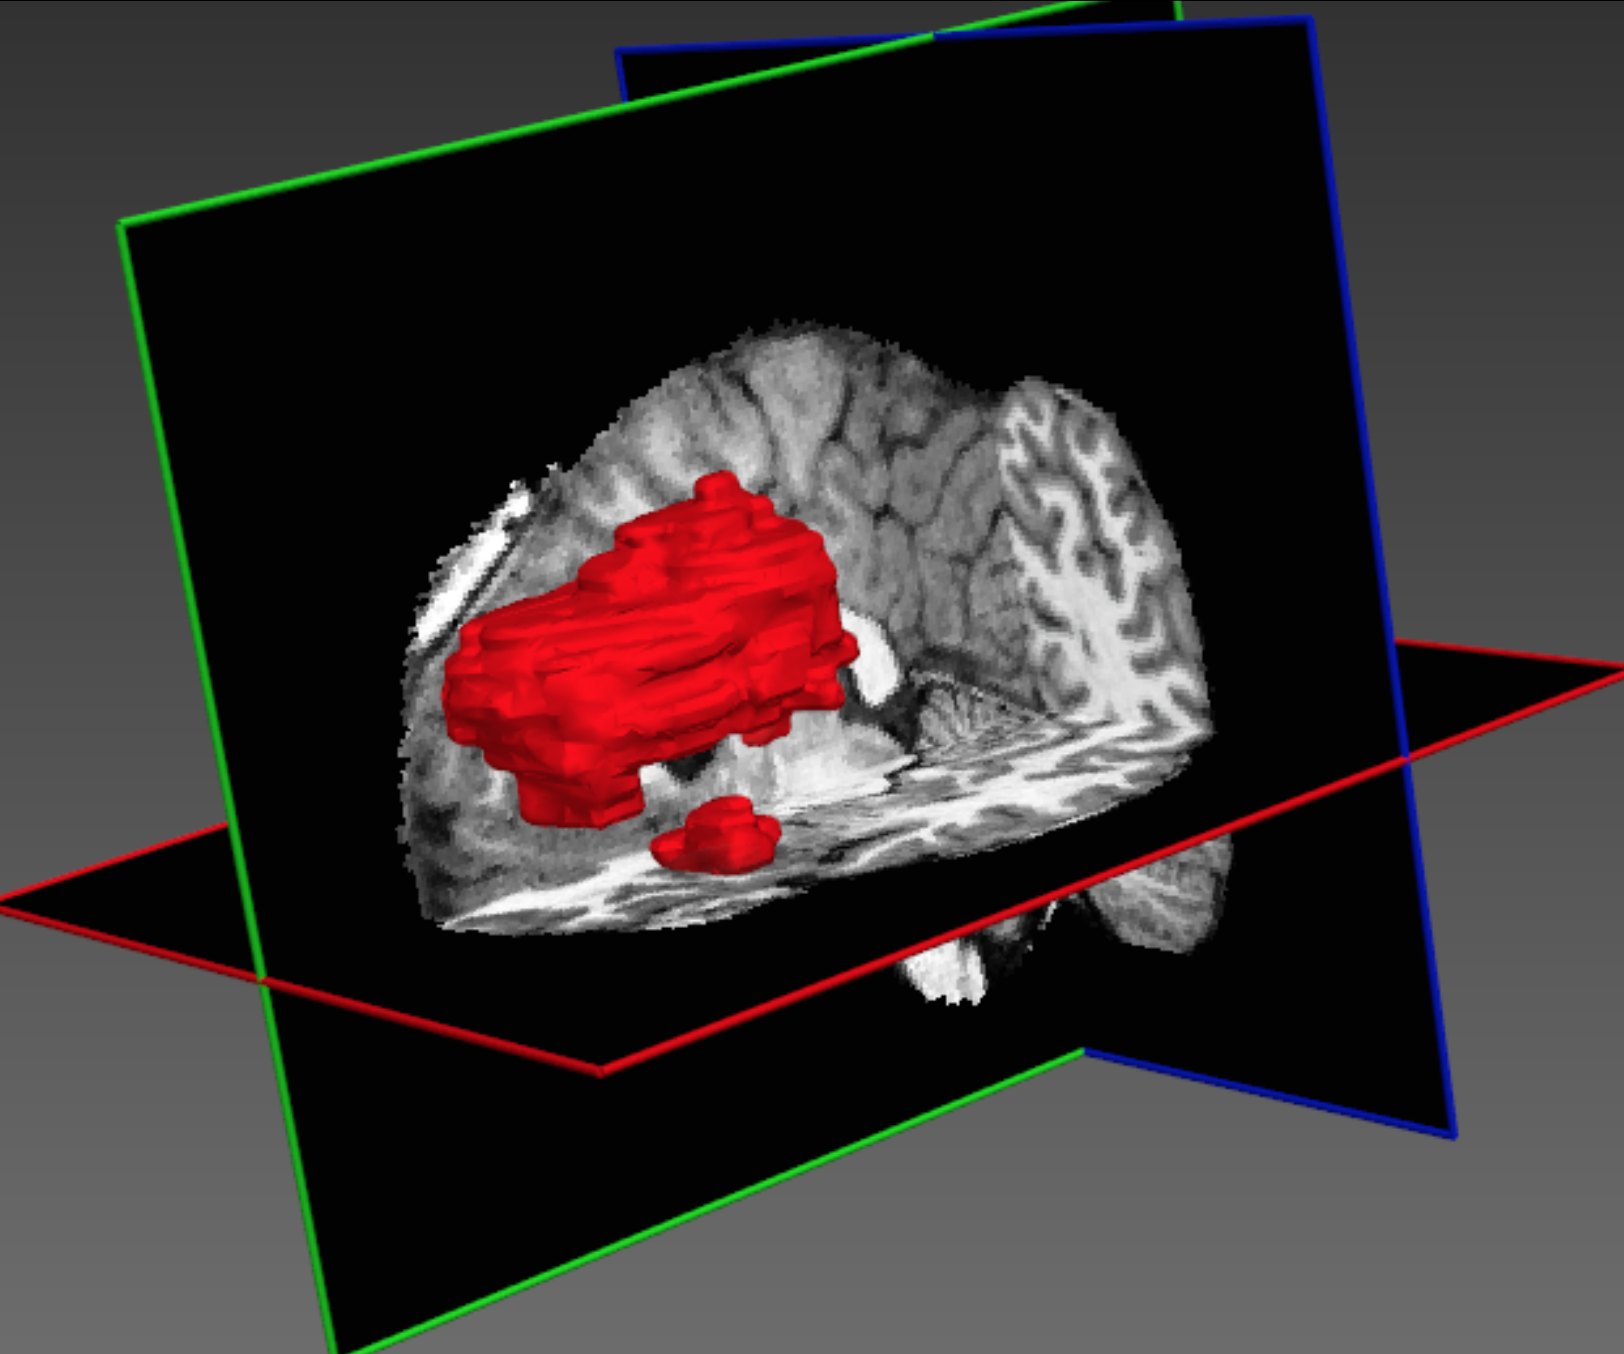
\includegraphics[clip=true, trim=10pt 0pt 10pt 0pt, width=1.\textwidth]{figures/introduction/3dLesionBig.png}
	\caption{}
	\label{fig:3dLesionBig}
\end{subfigure}
\begin{subfigure}[b]{0.225\textwidth}
	\centering
	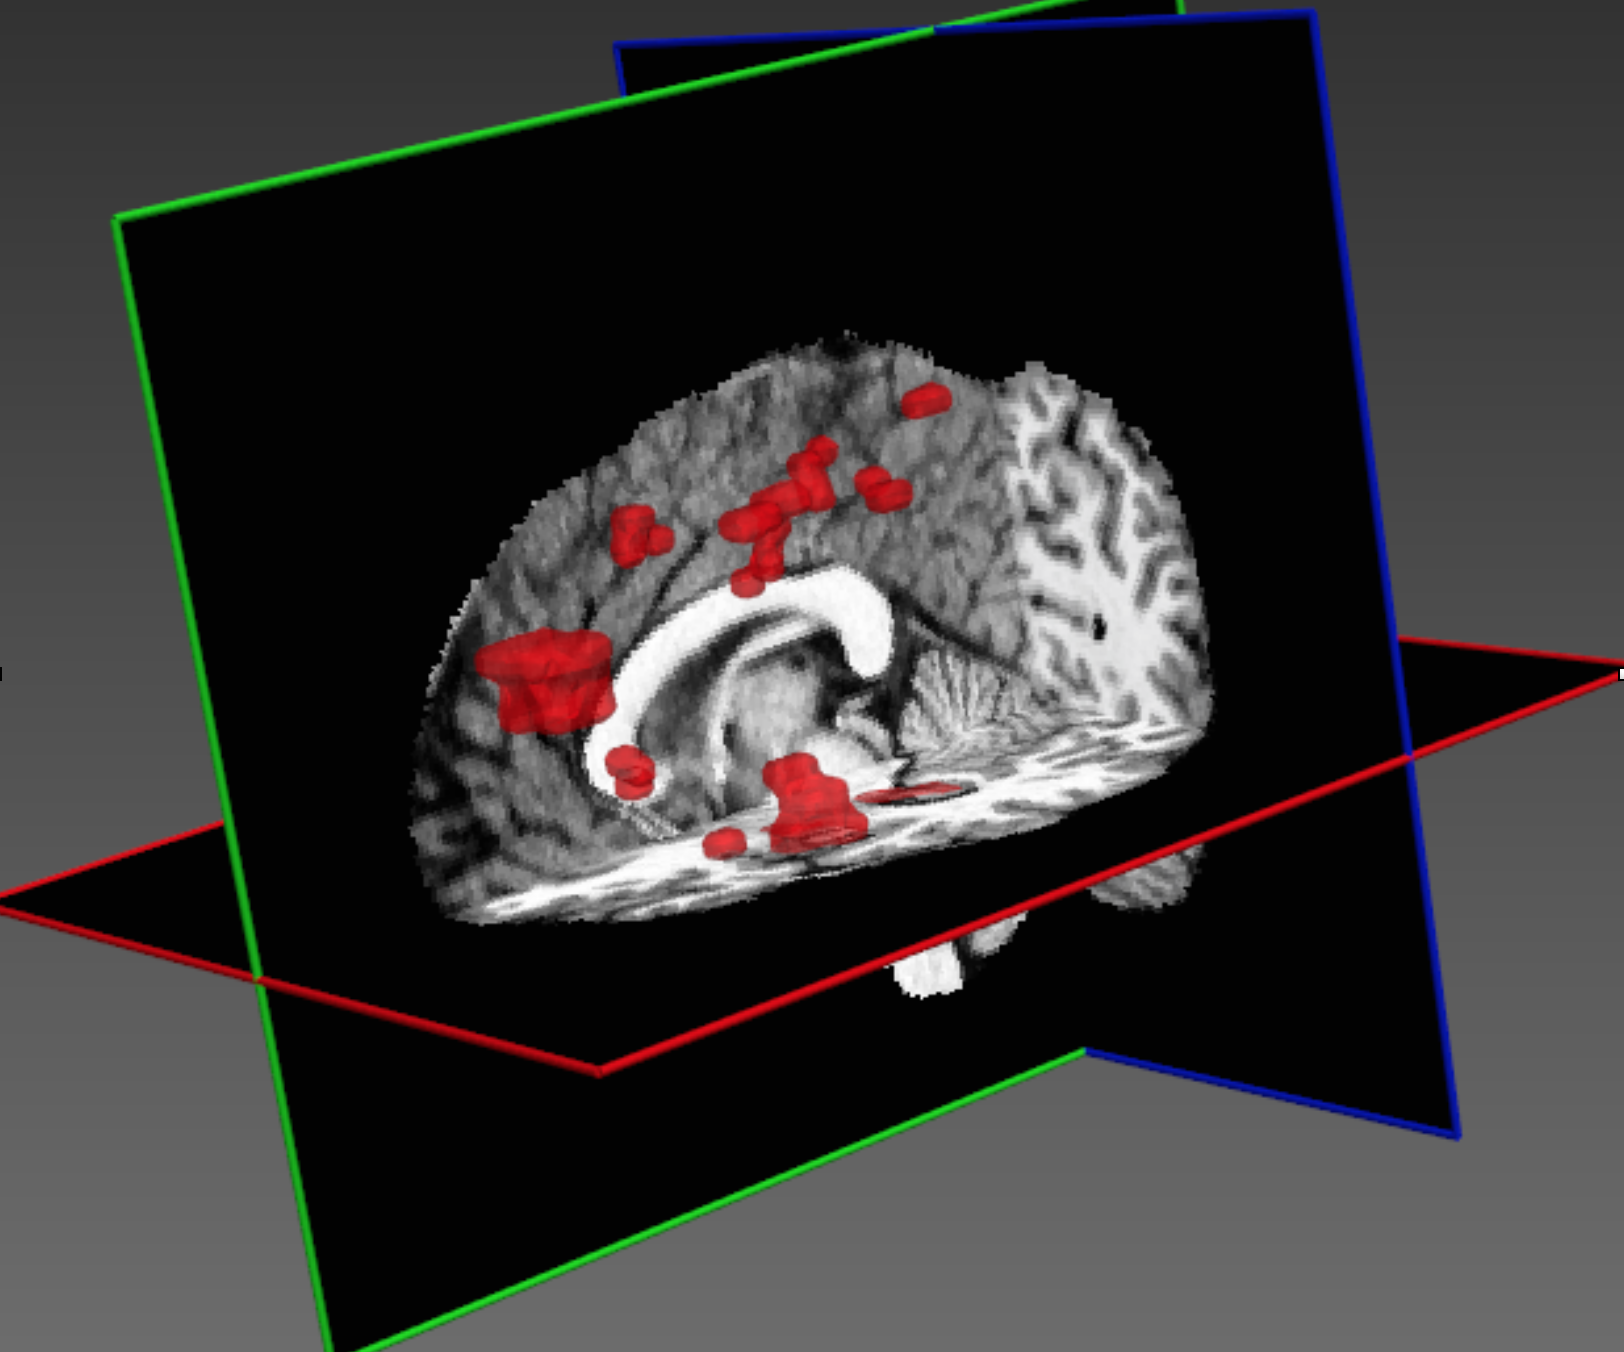
\includegraphics[clip=true, trim=10pt 0pt 10pt 0pt, width=1.\textwidth]{figures/introduction/3dLesionsSmalls.png}
	\caption{}
	\label{fig:3dLesionSmalls}
\end{subfigure}
\begin{subfigure}[b]{0.225\textwidth}
	\centering
	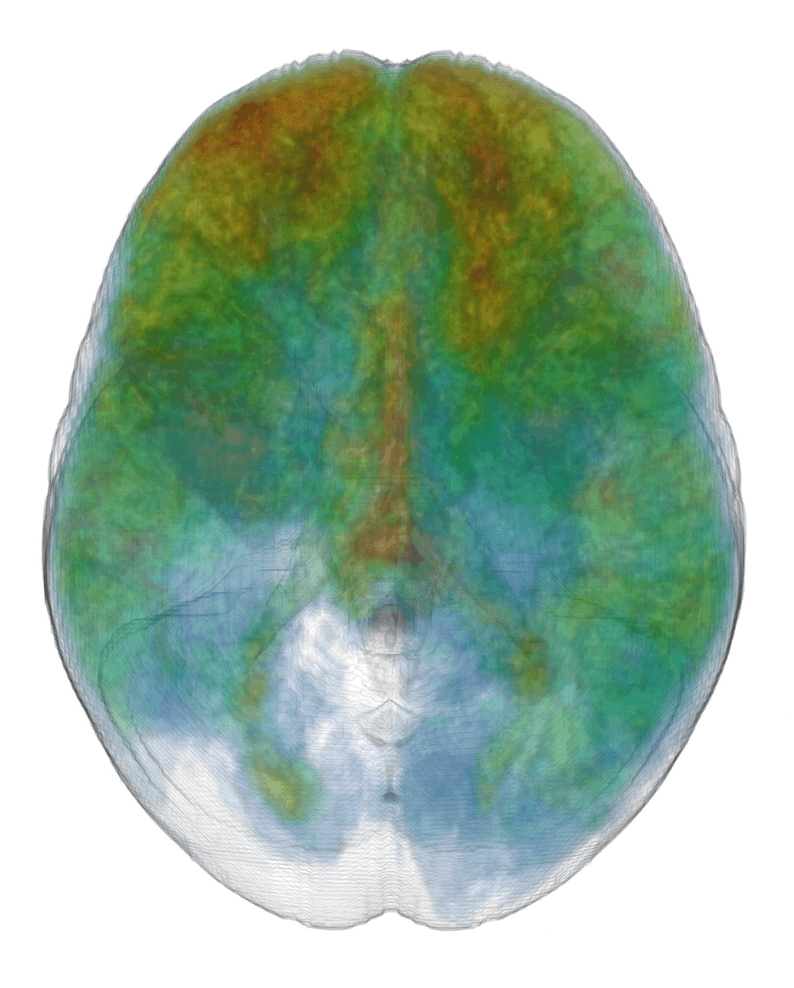
\includegraphics[clip=true, trim=10pt 20pt 10pt 20pt, width=0.7\textwidth]{figures/introduction/trio/top1Small.png}
	\caption{}
	\label{fig:spatialMap}
\end{subfigure}
\begin{subfigure}[b]{0.22\textwidth}
	\centering
	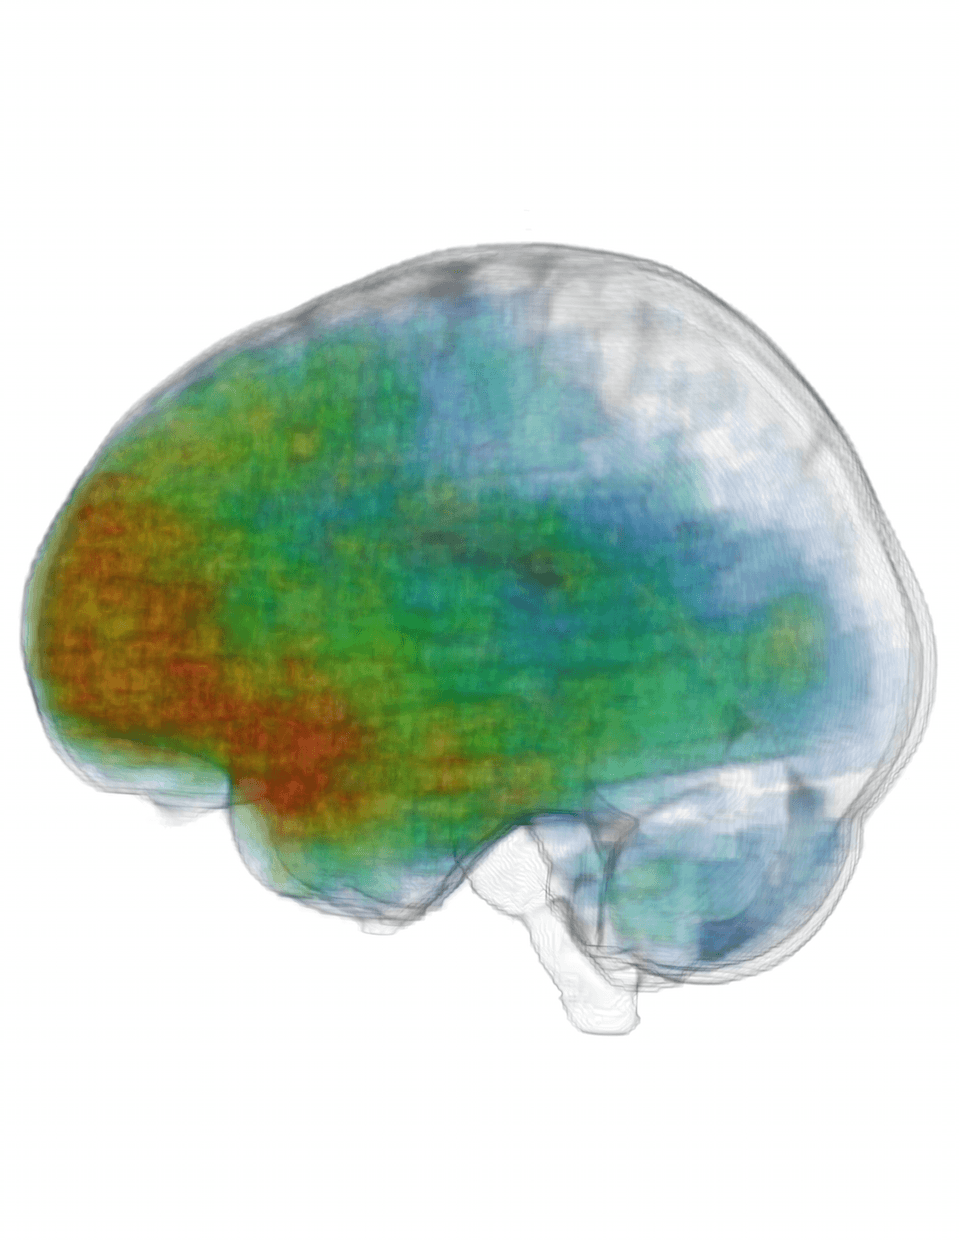
\includegraphics[clip=true, trim=0pt 190pt 0pt 0pt, width=1.0\textwidth]{figures/introduction/trio/side1Small.png}
	\caption{}
	\label{fig:spatialMapSide}
\end{subfigure}
%add desired spacing between images, e. g. ~, \quad, \qquad, \hfill etc.
%(or a blank line to force the subfigure onto a new line)
\\[1ex] %Break line. So that next figures go in their own line.
\centering
\begin{subfigure}[b]{1.0\textwidth}
\centering
	%\includegraphics[width=1.0\textwidth]{figures/figIntHistoWholeDataset/new13Mar/histoIntensGreenRedNoSupt.png}
	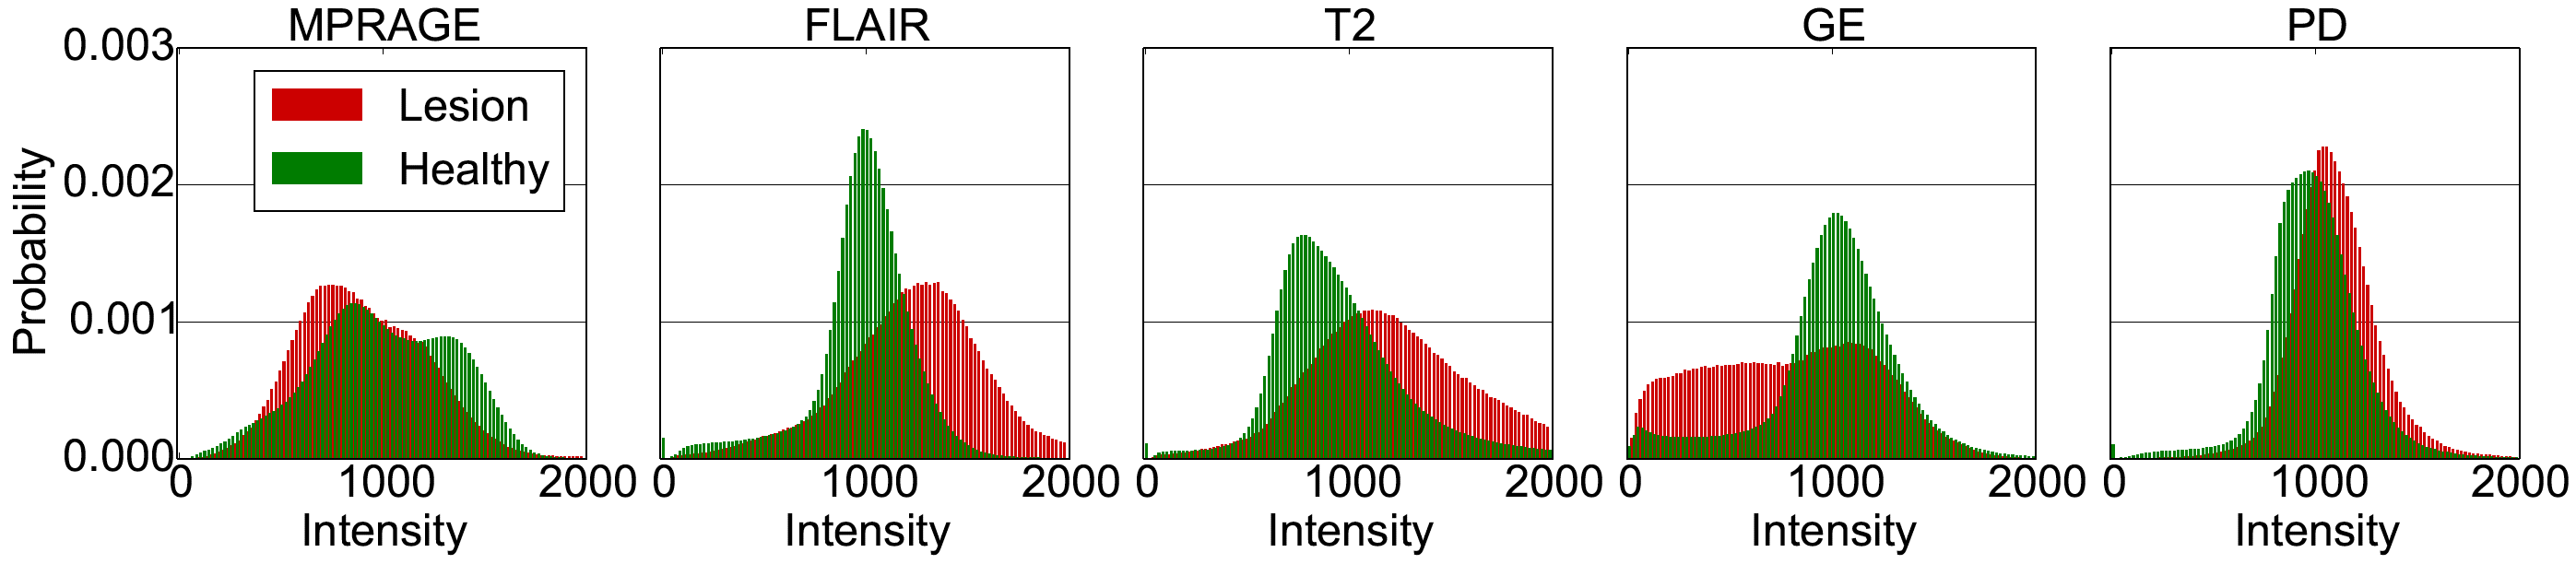
\includegraphics[clip=true, trim=0pt 0pt 0pt 0pt, width=1.0\textwidth]{figures/introduction/trio/intHistoTrio1_5mods.png}
	\caption{}
	\label{fig:histInt}
\end{subfigure}

\caption{Heterogeneous appearance of TBI lesions poses challenges in devising discriminative models. Lesion size varies significantly with both large, focal and small, diffused lesions (a,b). Alignment of manual lesion segmentations reveals the wide spatial distribution of lesions in (c,d) with some areas being more likely than others. (e) shows the average of the normalized intensity histograms of different MR channels over all the TBI cases in our database, for healthy (green) and injured (red) tissue. One can observe a large overlap between the distributions of healthy and non-healthy tissue.}
\label{fig:tbiChallenges}
\end{figure}

\subsection{Related Work}

A multitude of automatic lesion segmentation methods have been proposed over the last decade, and several main categories of approaches can be identified. One group of methods poses the lesion segmentation task as an abnormality detection problem, for example by employing image registration. The early work of \cite{Prastawa2004} and more recent ones by \cite{Schmidt2012} and \cite{doyle2013Brats} align the pathological scan to a healthy atlas and lesions are detected based on deviations in tissue appearance between the patient and the atlas image. Lesions, however, may cause large structural deformations that may lead to incorrect segmentation due to incorrect registration. \cite{Gooya2011,Parisot2012} alleviate this problem by jointly solving the segmentation and registration tasks. \cite{Liu2014} showed that registration together with a low-rank decomposition gives as a by-product the abnormal structures in the sparse components, although, this may not be precise enough for detection of small lesions. Abnormality detection has also been proposed within image synthesis works. Representative approaches are those of \cite{Weiss2013} using dictionary learning and \cite{Ye2013a} using a patch-based approach. The idea is to synthesize pseudo-healthy images that when compared to the patient scan allow to highlight abnormal regions. In this context, \cite{cardoso15} present a generative model for image synthesis that yields a probabilistic segmentation of abnormalities. Another unsupervised technique is proposed by \cite{Erihov2015}, a saliency-based method that exploits brain asymmetry in pathological cases. A common advantage of the above methods is that they do not require a training dataset with corresponding manual annotations. In general, these approaches are more suitable for detecting lesions rather than accurately segmenting them.

Some of the most successful, supervised segmentation methods for brain lesions are based on voxel-wise classifiers, such as Random Forests. Representative work is that of \cite{Geremia2010} on MS lesions, employing intensity features to capture the appearance of the region around each voxel. \cite{Zikic2012} combine this with a generative Gaussian Mixture Model (GMM) to obtain tissue-specific probabilistic priors (\cite{Leemput1999}). This framework was adopted in multiple works, with representative pipelines for brain tumors by \cite{tustison2013Brats} and TBI by \cite{Rao2014b}. Both works incorporate morphological and contextual features to better capture the heterogeneity of lesions. \cite{Rao2014b} also incorporate brain structure segmentation results obtained from a multi-atlas label propagation approach (\cite{Ledig2015}) to provide strong tissue-class priors to the Random Forests. \cite{tustison2013Brats} additionally use a Markov Random Field (MRF) to incorporate spatial regularization. MRFs are commonly used to encourage spatial continuity of the segmentation (\cite{Schmidt2012, Mitra2014}). Although those methods have been very successful, it appears that their modeling capabilities still have significant limitations. This is confirmed by the results of the most recent challenges \footnote{links: \href{http://braintumorsegmentation.org/}{http://braintumorsegmentation.org/}, \href{www.isles-challenge.org}{www.isles-challenge.org}}, and also by our own experience and experimentation with such approaches.  

At the same time, deep learning techniques have emerged as a powerful alternative for supervised learning with great model capacity and the ability to learn highly discriminative features for the task at hand. These features often outperform hand-crafted and pre-defined feature sets. In particular, Convolutional Neural Networks (CNNs) (\cite{LeCun1998, Krizhevsky2012}) have been applied with promising results on a variety of biomedical imaging problems. \cite{Ciresan2012} presented the first GPU implementation of a two-dimensional CNN for the segmentation of neural membranes. From the CNN based work that followed, related to our approach are the methods of \cite{zikic2014CnnBrats, Havei2015Journal, pereira2015Brats}, with the latter being the best performing automatic approach in the BRATS 2015 challenge (\cite{Menze2014}). These methods are based on 2D CNNs, which have been used extensively in computer vision applications on natural images. Here, the segmentation of a 3D brain scan is achieved by processing each 2D slice independently, which is arguably a non-optimal use of the volumetric medical image data. Despite the simplicity in the architecture, the promising results obtained by these methods indicate the potential of CNNs.

Fully 3D CNNs come with an increased number of parameters and significant memory and computational requirements. Previous work discusses problems and apparent limitations when employing a 3D CNN on medical imaging data (\cite{prasoon2013Knee, Li2014a, Roth2014}). To incorporate 3D contextual information, multiple works used 2D CNNs on three orthogonal 2D patches (\cite{prasoon2013Knee, Roth2014, lyksborg2015ensemble}). In their work for structural brain segmentation, \cite{Brebisson2015a} extracted large 2D patches from multiple scales of the image and combined them with small single-scale 3D patches, in order to avoid the memory requirements of fully 3D networks.

One of the reasons that discouraged the use of 3D CNNs is the slow inference due to the computationally expensive 3D convolutions. In contrast to the 2D/3D hybrid variants (\cite{Roth2014, Brebisson2015a}), 3D CNNs can fully exploit \textit{dense-inference} (\cite{LeCun1998,Sermanet2013}), a technique that greatly decreases inference times and which we will further discuss in section \ref{subsec:theBaseline}. By employing dense-inference with 3D CNNs, \cite{Brosch2015} and \cite{urban2014CnnBrats} reported computation times of a few seconds and approximately a minute respectively for the processing of a single brain scan. Even though the size of their developed networks was limited, a factor that is directly related to a network's representational power, their results on MS and brain tumor segmentation respectively were very promising.

Performance of CNNs is significantly influenced by the strategy for extracting training samples. A commonly adopted approach is training on image patches that are equally sampled from each class. This, however, biases the classifier towards rare classes and may result in over-segmentation. To counter this, \cite{Ciresan2013} proposes to train a second CNN on samples with a class distribution close to the real one, but oversample pixels that were incorrectly classified in the first stage. A secondary training stage was also suggested by \cite{Havei2015Journal}, who retrain the classification layer on patches extracted uniformly from the image. In practice, two stage training schemes can be prone to overfitting and sensitive to the state of the first classifier. Alternatively, \textit{dense training} (\cite{Long2014}) has been used to train a network on multiple or all voxels of a single image per optimisation step (\cite{urban2014CnnBrats, Brosch2015, Ronneberger2015}). This can introduce severe class imbalance, similarly to uniform sampling. Weighted cost functions have been proposed in the two latter works to alleviate this problem. \cite{Brosch2015} manually adjusted the sensitivity of the network, but the method can become difficult to calibrate for multi-class problems. \cite{Ronneberger2015} first balance the cost from each class, which has an effect similar to equal sampling, and further adjust it for the specific task by estimating the difficulty of segmenting each pixel.

\subsection{Contributions}

We present a fully automatic approach for lesion segmentation in multi-modal brain MRI based on an 11-layers deep, multi-scale, 3D CNN with the following main contributions:

\begin{enumerate}

\item We propose an efficient hybrid training scheme, utilizing \textit{dense training} (\cite{Long2014}) on sampled image segments, and analyze its behaviour in adapting to class imbalance of the segmentation problem at hand.

\item We analyze in depth the development of deeper, thus more discriminative, yet computationally efficient 3D CNNs. We exploit the utilization of small kernels, a design approach previously found beneficial in 2D networks (\cite{Simonyan2014}) that impacts 3D CNNs even more, and present adopted solutions that enable training deeper networks. 

\item We employ parallel convolutional pathways for multi-scale processing, a solution to efficiently incorporate both local and contextual information which greatly improves segmentation results.

\item We demonstrate the generalization capabilities of our system, which without significant modifications outperforms the state-of-the-art on a variety of challenging segmentation tasks, with top ranking results in two MICCAI challenges, ISLES and BRATS.

\end{enumerate}

Furthermore, a detailed analysis of the network reveals valuable insights into the powerful black box of deep learning with CNNs. For example, we have found that our network is capable of learning very complex, high level features that separate gray matter (GM), cerebrospinal fluid (CSF) and other anatomical structures to identify the image regions corresponding to lesions.

Additionally, we have extended the fully-connected Conditional Random Field (CRF) model by \cite{Krahenbuhl2013} to 3D which we use for final post-processing of the CNN's soft segmentation maps. This CRF overcomes limitations of previous models as it can handle arbitrarily large neighborhoods while preserving fast inference times. To the best of our knowledge, this is the first use of a fully connected CRF on medical data.

To facilitate further research and encourage other researchers to build upon our results, the source code of our lesion segmentation method including the CNN and the 3D fully connected CRF is made publicly available on \url{https://biomedia.doc.ic.ac.uk/software/deepmedic/}.

